\documentclass[31pt]{article}
\setlength{\columnsep}{0.13\columnwidth}
%\setlength{\columnseprule}{0.05\columnwidth}
 
\usepackage{geometry}
\geometry{left=2.3cm, right=2.3cm, top=2.5cm, bottom=2.5cm}

\usepackage{fontspec}
\setmainfont{Times New Roman}

\usepackage{xeCJK}

\usepackage{subfigure}

\usepackage{amssymb}

\usepackage{amsmath}

\usepackage{graphicx}

\usepackage{booktabs}

\usepackage{longtable}

\usepackage{tabularx}

\usepackage{wrapfig}

\usepackage{indentfirst}

\usepackage{bm}								%粗斜体

\usepackage{float}								%超级好用!浮动排版!

\usepackage{flushend,cuted}
 
\usepackage{caption}
\captionsetup{font={scriptsize}}						%改变图名字体大小

\usepackage{subfig}
\captionsetup[subfigure]{labelformat=simple, listofformat=subsimple, farskip = 0pt}

\usepackage{hyperref}							%超链接!

\usepackage{fancyhdr}

\usepackage{stfloats}

\setlength{\parindent}{2em}

\linespread{1.2}

\usepackage{ragged2e}             %两端对齐!

\usepackage{algorithm}

\usepackage{algorithmicx}

\usepackage{algpseudocode}

\renewcommand{\algorithmicrequire}{\textbf{Input:}}  % Use Input in the format of Algorithm
\renewcommand{\algorithmicensure}{\textbf{Output:}} % Use Output in the format of Algorithm

\begin{document}

\title{EE450 Introduction to Computer Networks - Fall 2019 - HW 3}
\author{Junzhe Liu,\; 2270250947}

\begin{document}

\maketitle

\pagestyle{fancy}
\lhead{}
\rhead{\textbf{\thepage}}
\chead{\textit{ Junzhe Liu / 2270250947 / Viterbi School of Engineering, Computer Science}}
\lfoot{}
\cfoot{}
\rfoot{}

\section{Reading Assignment:}

\justifying\large Chapter 6

\section{Problems to be solved:}

\subsection{Chapter 6, Page 507: R1 Consider the transportation analogy in Section 6.1.1. If the passenger is analogous to a datagram, what is analogous to the link layer frame?}

The Transportation mode, for instance, car, bus, train, boat, plane, etc.



\subsection{Chapter 6, Page 507: R5 In Section 6.3, we listed four desirable characteristics of a broadcast channel. Which of these characteristics does slotted ALOHA have? Which of these characteristics does token passing have?}

Slotted ALOHA: 1, 2, and 4. Slotted ALOHA is partially decentralized, since it requires the clocks of all nodes to be synchronized.

Token passing: All 4 characteristics.


\subsection{Chapter 6, Page 508: P2 Show (give an example other than the one in Figure 6.5) that two-dimensional parity checks can correct a single bit error. Show (give an example of) a double-bit error that can be detected but not corrected.}

\begin{figure}[H]
\centering
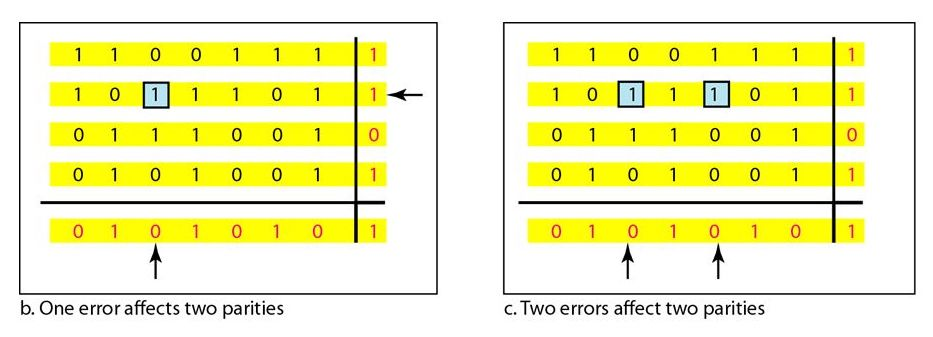
\includegraphics[scale=0.38]{1.jpg}
\caption{Left: single bit error detection and correction. Right: double-bit error can be detected but not corrected.}
\end{figure}

The above images show two situations. In the left image, suppose that the bit in the blue frame flips into 0, two-dimensional parity check can quickly locate the error by checking the parity bit number. 

However in the right image, suppose two 1s in both blue frame flips into 0, two-dimensional parity check can find out that the error locates on column 3 and 5, but cannot know which row exactly; This is because two errors take place on the same row, and do not change the parity of the row 2, therefore it can only detect two bit errors but cannot correct them.


\subsection{Chapter 6, Page 509: P5 Consider the 5-bit generator, G = 10011, and suppose that D has the value 1010101010. What is the value of R? }

We divide $(D\cdot2^4)=(1010101010,0000)$ by $G=10011$, the remainder will be:

\begin{equation}
10101010100000 / 10011 = 1011011100\;\; \mathrm{mod}\;\; 0100
\end{equation}

so $R=0100$, the complete message will be $(1010101010,0100)$.


\subsection{Chapter 6, Page 509: P7 In this problem, we explore some of the properties of the CRC. For the generator G (= 1001) given in Section 6.2.3, answer the following questions.}

\subsubsection{Why can it detect any single bit error in data D?}

Without loss of generality, suppose $G$ has $r$ bits and $D$ has $d$ bits. $D$ will be padded with $r-1$ zeros. Suppose the remainder of $D\cdot2^{r-1} / G$ is $R$, the whole message will be $D\cdot2^{r-1} + R$.

We now suppose that the $i$-th bit is flipped: $1\leq i \leq d+r-1$ and we assume that the rightmost bit is the first bit, then the message turns out to be: $M=D\cdot2^{r-1} + R \;\mathrm{XOR}\;2^{i-1}$. If we divide $M$ by $G$, the reminder will not be zero. Therefore the single bit can be detected.

\subsubsection{Can the above $G$ detect any odd number of bit errors? Why?}

Any number comprised of odd-number of 1s cannot by divided by 11, thus a number of odd-number bit errors also cannot be divided by 11. But $G$ can be divided by 11, thus $G$ can detect any odd number of bit errors.

\end{document}